\documentclass[oneside]{book}

\usepackage[utf8]{inputenc}
\usepackage[english]{babel}

\usepackage{titlesec}
\usepackage{fancyhdr}
\usepackage{graphicx}
\usepackage{caption}

\usepackage[a4paper, total={6in, 8in}]{geometry}
\usepackage{setspace}

\usepackage{amssymb}
\usepackage{amsmath}
\usepackage{mathtools}
\usepackage{adforn}

\usepackage{cancel}
\usepackage{array}
\usepackage{environ}
\usepackage{textcomp}

\usepackage{minted}
\usepackage{upquote}

\usepackage{hyperref}

\usepackage{apacite}

\let\CardinalNumeric\relax
\usepackage{amsrefs}
\usepackage{xpatch}
\xpatchcmd{\bibchapter}{*}{}{}{}
%\usepackage{calrsfs}
%\DeclareMathAlphabet{\pazocal}{OMS}{zplm}{m}{n}

\title{The Engineering of Subtraction}
\author{Liam Gardner}
\date{\today}

\graphicspath{ {figs/} }

\hypersetup{
    colorlinks,
    citecolor=black,
    filecolor=black,
    linkcolor=blue,
    urlcolor=black
}

\titleformat
{\chapter} % command
[display] % shape
{\bfseries\Large\itshape} % format
%{Story No. \ \thechapter} % label
{}
{0ex} % sep
{
    \rule{\textwidth}{1pt}
    \vspace{1ex}
    \centering
} % before-code
[
\vspace{-1.8ex}%
\rule{\textwidth}{1pt}
] % after-code

\renewcommand{\chaptermark}[1]{%
\markboth{#1}{}}
\pagestyle{fancy}
\fancyhf{}
\fancyhead[LE,RO]{The Engineering of Subtraction}
%\fancyfoot[CE,CO]{\leftmark}
%\fancyfoot[LE,RO]{\thepage}
\cfoot{\thepage}

\onehalfspace

\begin{document}

\newcommand{\Mod}[1]{\ (\mathrm{mod}\ #1)}
\newcommand{\Sub}{\mbox{\large $\mathrlap{\mathfrak{D}}\,\dag\,$}}
\newcommand{\GreaterThan}{\mbox{\large $\mathrlap{\mathfrak{P}}{\adfS}\,$}}
\newcommand{\LessThan}{\mbox{\large $\mathrlap{\mathfrak{L}}{\adfS}\,$}}
\newcommand\tab[1][1cm]{\hspace*{#1}}
\newcommand\hadd{\mbox{\large \textsection}}
\newcommand\newchapter[1]{%
\chapter{#1}
\markboth{#1}{}
\fancyhead[RE,LO]{\thechapter: #1}}
\maketitle
\tableofcontents
\newchapter{An interview with subtraction}
\tab
Subtraction is taught at a very basic level. Here in Canada, it's taught roughly in grade one or two. One of the things that always confused me was the concept of borrowing. Looking back on it, I'm less so confused, but more so disturbed by the way it was taught. As an example, let's go through the following subtraction statement.
\begin{center}
\begin{tabular}{c c c c c}
& 1 & 2 & 2 & 4 \\
- & & 6 & 4 & 3 \\
\end{tabular}
\end{center}
\tab
The algorithm works by starting from the rightmost digit, which in this instance is $4-3$, and perform the basic subtraction under the circumstance that the minuend (the first number) is greater than the subtrahend (the second number). In this case, we can see that this is true, and perform the subtraction to attain a value of 1.
\begin{center}
\begin{tabular}{c c c c c}
& 1 & 2 & 2 & 4 \\
- & & 6 & 4 & 3 \\
\hline
& & & & 1 \\
\end{tabular}
\end{center}
\tab
Moving to our next value, we can see that $2-4$ does not meet the requirement. As a standalone operation, $2-4=-2$. However, this is not standalone, and is instead based around a bigger ``problem''. In school, we are taught to perform something called \textit{borrowing}. This is when you usurp a value from the successive digit and add 10 to the digit we're working with. In our case, the successive digit is $2$. The algorithm tells us to subtract $1$ from the successive value, and add $10$ to the current value we're working with. This is the concept of borrowing. Now, we can proceed with the basic subtraction. $12-4 = 8$. Therefore, the next digit in our difference is $8$.
\begin{center}
\begin{tabular}{c c c c c}
& 1 & \xcancel{2}1 & 12 & 4 \\
- & & 6 & 4 & 3 \\
\hline
& & & 8 & 1 \\
\end{tabular}
\end{center}
\tab
When I first learned this, it wasn't just unintuitive to me, I was completely incapable of understanding what was happening. This algorithm for subtraction requires the performer to understand how to subtract two numbers normally. For a computer, this is completely fine, however as a method for teaching children, it was a nightmare. Furthermore, most elementary teachers can't go into too much detail as to how this algorithm works, it was ingrained into their brain and they were told to ingrain it into ours. For now, I'll complete the table with each step before continuing.
\begin{center}
\begin{tabular}{c c c c c}
& \xcancel{1}0 & 11 & 12 & 4 \\
- & & 6 & 4 & 3 \\
\hline
& & 5 & 8 & 1 \\
\end{tabular}
\end{center}
\begin{center}
\begin{tabular}{c c c c c}
& 1 & 2 & 2 & 4 \\
- & & 6 & 4 & 3 \\
\hline
& & 5 & 8 & 1 \\
\end{tabular}
\end{center}
\newchapter{Subtraction via modular arithmetic}
\tab
\textbf{I would like to start this section by saying that this has no immediately visible applications as to what we have been taught, but instead exists only to provide insight as to the concept of subtraction's borrowing.} To begin, let's take a look at modular arithmetic in base 10. The modulo operator works by taking the remainder of the division by 10. That is, for any function $f(x)$, $f(x)\mathrm{\,\,mod\,\,} 10$ is the same as saying  ``divide $f(x)$ by 10, and return the remainder.'' For some basic pretense, $\forall x \in [0,10), x\mathrm{\,\,mod\,\,}10 = x$. Here are some more values in what is known as $\mathbb{Z}_10$.

\begin{center}
\begin{tabular}{|c|c|c|c|c|c|}
\hline
x values & -5 & -4 & -3 & -2 & -1 \\
\hline
$x$ mod 10 & 5 & 6 & 7 & 8 & 9\\
\hline
x values & 11 & 12 & 13 & 14 & 15\\
\hline
$x$ mod 10 & 1 & 2 & 3 & 4 & 5\\
\hline
x values & -30 & -29 & -28 & -27 & -26 \\
\hline
$x$ mod 10 & 0 & 1 & 2 & 3 & 4 \\
\hline 
\end{tabular}
\end{center}
\tab
All numbers will wrap around to end up on the interval $[0,10)$. Calculations that end with the result mod 10 can be said to be part of a set called $\mathbb{Z}_{10}$. This is because all all output values will end up in the interval $[0,10)$. Typically, operations in integer rings such as $\mathbb{Z}_{10}$ will only have inputs in that interval as well. Since digit subtraction will always have the minuend and subtrahend be within that interval, it wouldn't be incorrect to say that they take place in the integer ring $\mathbb{Z}_{10}$. In later sections, we will be moving into the binary system, which means operations will exist in the integer ring $\mathbb{Z}_2$ rather than $\mathbb{Z}_{10}$, and all values will exist on the interval $[0,2)$. 
\newline
\tab
A different subtraction algorithm can be created as follows:
\begin{itemize}
	\item Align subtraction vertically, in the same way as the conventional algorithm.
	\item We read from right to left. Start with the two rightmost digits.
	\item Perform the single-digit subtraction.
	\item Take the calculated difference, mod 10 and write that digit below your aligned numbers.
	\item If the minuend was less than the subtrahend, place an indicator above the successive digits.
	\item Repeat process for all remaining digits.
	\item For all digits with an indicator above them, subtract 1 from the final digit.
	\item The remaining value is your difference. All numbers with indicators above them had been borrowed from.
\end{itemize}
\tab
For the time being, we'll call this algorithm \textit{modular subtraction}. This new algorithm fixes two problems: the first is that it removes the problem I had with having two-digit numbers in places meant to hold one digit (which probably shouldn't be considered an objective problem). The second is a problem that I haven't spoken of yet. Using the normal subtraction algorithm, subtracting numbers $2n-n,\, n \in \mathbb{N} \mid \{5\leq n < 10\}$ will end up with repetition. As an example, let's take a look at subtracting $10-5$ and $18-9$.
\begin{center}
\setlength{\tabcolsep}{1pt}
\begin{tabular}{c c c}
 & 1 & 0 \\
- & & 5\\
\end{tabular}
\end{center}
\tab
As per the normal subtraction algorithm, since $0 < 5$, we borrow from the successive digit. This process will result in the following
\begin{center}
\setlength{\tabcolsep}{2.5pt}
\begin{tabular}{c c c}
&\xcancel{1}0 & 10 \\
-&&5 \\
\end{tabular}
\end{center}
\tab
We end up in this loop, having to repeat this process infinitely. As a result, most children will learn to memorize the answers to certain problems like this. As another example, here's what happens with $18-9$.
\begin{center}
\setlength{\tabcolsep}{1pt}
\begin{tabular}{c c c}
&1&8\\
-&&9\\
\end{tabular}
\end{center}
\begin{center}
\setlength{\tabcolsep}{2.5pt}
\begin{tabular}{c c c}
 &\xcancel{1}0 & 18\\
-& & 9\\
\end{tabular}
\end{center}
\tab
We'll get to solving this problem with modular subtraction later. For now, let's take a look at our original problem. The first step is to re-create the same setup we'd use conventionally.
\begin{center}
\begin{tabular}{c c c c c}
& 1 & 2 & 2 & 4 \\
- & & 6 & 4 & 3
\end{tabular}
\end{center}
\tab
Next, we look at and subtract the rightmost two digits. $4-3=1$. Now, we take the remainder of that difference when divided by 10. $1\Mod{10} = 1$. So, we put a $1$ as the rightmost digit to our answer. Since the minuend was greater than the subtrahend, we don't have to place an indicator above the next digit.
\begin{center}
\begin{tabular}{c c c c c}
& 1 & 2 & 2 & 4 \\
- & & 6 & 4 & 3 \\
\hline
& & & & 1
\end{tabular}
\end{center}
\tab
Next, we move on and look at the digits $2$ and $4$. $2-4=-2$. $-2\Mod{10}=8$. Our next digit is 8. Since $2<4$, we place an indicator above the next digit.
\begin{center}
\begin{tabular}{c c c c c}
& & \textreferencemark & & \\
& 1 & 2 & 2 & 4 \\
- & & 6 & 4 & 3 \\
\hline
& & & 8 & 1
\end{tabular}
\end{center}
\tab
I'm using \textreferencemark, often called the \textit{komejirushi} (meaning rice symbol), \textit{reference mark}, \textit{reference symbol}. Since I'm most familiar with it being called the komejirushi, I'll stick to that for this document. However, it's worth noting that however you indicate borrowing is up to you, and can be done in more ways than just placing a symbol above the column. Moving on, we calculate the modular difference for the digits $2$ and $6$. We see that $2-6=-4$. $-4\Mod{10}=6$. Since we have the borrow indicator in this column, we subtract one from this value, making the next digit $5$ rather than $6$. Along with that, we see that the minuend in this case is smaller than the subtrahend, and so we place another indicator above the next column.
\begin{center}
\begin{tabular}{c c c c c}
& \textreferencemark & \textreferencemark & & \\
& 1 & 2 & 2 & 4 \\
- & & 6 & 4 & 3 \\
\hline
& & 5 & 8 & 1
\end{tabular}
\end{center}
\tab
Repeating the same process, $1-0=1$. $1\Mod{10}=1$. Since there's the borrow indicator, we subtract $1$ from this value, making this last digit $0$. Therefore, the final result is $581$, which aligns with the conventional algorithm.
\newline
\tab
This algorithm fixes my initial problem of not liking how the alignment of digits breaks when borrowing in the original algorithm, as well as the recursion error with $2n-n$ subtraction. If we were to use modular subtraction to solve $18-9$, We would proceed as follows, (ignoring the alignment step): $8-9=-1$, $-1\Mod{10}=9$, our first digit is 9 and since $8<9$, we place an indicator on the next digit. $1-0=1$, $1\Mod{10}=1$, $1-1=0$. Therefore, our final answer is $9$ and we avoided a recursive loop.


\newchapter{Subtraction in binary and the half-subtractor}
\label{chap:halfsub}
\tab
For now, let's go through single-bit subtraction limiting our inputs to 0 and 1.
\begin{center}
\begin{tabular}{|c|c|c|c|}
\hline
$x$ & $y$ & $x-y$ & $b$ \\
\hline
0 & 0 & 0 & \\
\hline
0 & 1 & -1 & \textreferencemark \\
\hline
1 & 0 & 1 & \\
\hline
1 & 1 & 0 & \\
\hline
\end{tabular}
\end{center}
\tab
I've added an extra $b$ column that indicates negativity. This might seem a bit unnecessary, since there's only one way to get a negative number in these permutations. However, I'll leave it there nonetheless. In binary, the only digits we have access to are $0$ and $1$, and so to restrict our outputs to that, and so we'll operate in $\mathbb{Z}_2$. As a result, we'll take the difference mod 2. This produces the following table. Note that in this table $q=x-y$. We can interpret the $b$ column as a boolean representing the presence of negativity. Since all but one numbers is positive, most values will be 0.
\begin{center}
\begin{tabular}{|c|c|c|c|}
\hline
$x$ & $y$ & $q\Mod{2}$ & $b$ \\
\hline
0 & 0 & 0 &0 \\
\hline
0 & 1 & 1 & 1 \\
\hline
1 & 0 & 1 & 0\\
\hline
1 & 1 & 0 & 0\\
\hline
\end{tabular}
\end{center}
\tab
Since our goal is to mimic this with circuitry, we'll have to represent the outputs using boolean logic. The first output column of $q\Mod{2}$ is obviously the $\mathcal{XOR}$ gate. The second output $b$ is a little hard to figure out. For now, let's take a look at the three main truth tables ($\mathcal{XOR}$ is compositional)
\begin{center}
\begin{tabular}{ |c|c|c| }
 \hline
 \multicolumn{3}{|c|}{$\mathcal{OR}$} \\
 \hline
 $a$ & $b$ & $_a\mathcal{OR}_b$ \\
 \hline
 0 & 0 & 0\\
 0 & 1 & 1\\
 1 & 0 & 1\\
 1 & 1 & 1\\
 \hline
\end{tabular}
\tab
\begin{tabular}{ |c|c| }
 \hline
 \multicolumn{2}{|c|}{$\mathcal{NOT}$} \\
 \hline
 $a$ & $\overline{a}$ \\
 \hline
 0 & 1\\
 1 & 0\\
 \hline
\end{tabular}
\tab
\begin{tabular}{ |c|c|c| }
 \hline
 \multicolumn{3}{|c|}{$\mathcal{AND}$} \\
 \hline
 $a$ & $b$ & $_a\mathcal{AND}_b$ \\
 \hline
 0 & 0 & 0\\
 0 & 1 & 0\\
 1 & 0 & 0\\
 1 & 1 & 1\\
 \hline
\end{tabular}
\end{center}
\tab
Since most of this document uses standard mathematical symbols, the logical operators will not be represented using overlapping symbols. In other words $a+b$ in logic will be written as $_a\mathcal{OR}_b$ instead. This notation is similar to how the combination and permutation function are written occasionally, and so I doubt this will generate any confusion. In case things get messy, I may also use functional notation instead: $\mathcal{AND}(a,b)$.
\newline
\tab
Applying the not operator to the and gate will invert all bits, making $\overline{_1\mathcal{AND}_1}$ the only output to be 0. That output corresponds with the output value in the $b$ column from earlier. Along with that $\overline{_0\mathcal{AND}_1}$ outputs 1, which was also a goal of ours. However, as for the other two outputs, they both aren't what we're looking for. The two outputs we're looking for are also shared with the $\mathcal{OR}$ gate. The $\mathcal{OR}$ gate also holds the property of outputting 0 when both inputs are 0, something lacking in our $\overline{\mathcal{AND}}$ gate. We can thus construct the following expression and truth table
$$
\mathcal{AND}(\overline{_a\mathcal{AND}_b},\, _a\mathcal{OR}_b)
$$
\begin{center}
\begin{tabular}{|c|c|c|}
\hline
$a$ & $b$ & $q$ \\
\hline
0 & 0 & 0 \\
\hline
0 & 1 & 1 \\
\hline
1 & 0 & 1 \\
\hline
1 & 1 & 0 \\
\hline
\end{tabular}
\end{center}
\tab
This is an equation representing the $\mathcal{XOR}$ gate. The reason we've written this out is because now we can use the boolean algebraic laws to expand our expression into the following.
$$
\mathcal{OR}(_{\overline{a}}\mathcal{AND}_b,\,_{a}\mathcal{AND}_{\overline{b}})
$$
\tab
We can now break this down into two parts, the first is $_{\overline{a}}\mathcal{AND}_b$, and the second is $_a\mathcal{AND}_{\overline{b}}$. The truth tables for these are as follows.
\begin{center}
\begin{tabular}{|c|c|c|}
\hline
\multicolumn{3}{|c|}{$_{\overline{a}}\mathcal{AND}_b$} \\
\hline
$a$ & $b$ & $q$ \\
\hline
0 & 0 & 0 \\
\hline
0 & 1 & 1 \\
\hline
1 & 0 & 0 \\
\hline
1 & 1 & 0 \\
\hline
\end{tabular}
\tab
\begin{tabular}{|c|c|c|}
\hline
\multicolumn{3}{|c|}{$_a\mathcal{AND}_{\overline{b}}$} \\
\hline
$a$ & $b$ & $q$ \\
\hline
0 & 0 & 0 \\
\hline
0 & 1 & 0 \\
\hline
1 & 0 & 1 \\
\hline
1 & 1 & 0 \\
\hline
\end{tabular}
\end{center}
\tab
It is clear now, that the equation we're looking for to represent the presence of negativity is $_{\overline{a}}\mathcal{AND}_b$. From here, we can form a proper understanding of logical subtraction. Note that the word ``borrow'' in this case represents the presence of negativity.

\begin{center}
\begin{tabular}{|c|c|c|c|}
\hline
$\mathrm{bit}_1$ & $\mathrm{bit}_2$ & difference & borrow \\
\hline
$x$ & $y$ & $_x\mathcal{XOR}_y$ & $_{\overline{x}}\mathcal{AND}_y$ \\
\hline
0 & 0 & 0 &0 \\
\hline
0 & 1 & 1 & 1 \\
\hline
1 & 0 & 1 & 0\\
\hline
1 & 1 & 0 & 0\\
\hline
\end{tabular}
\end{center}
\begin{figure}[h]
\centering
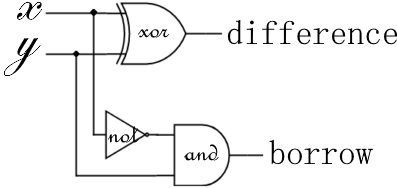
\includegraphics[scale=0.75]{halfsub}
\captionsetup{labelformat=empty}
\caption{Figure 1: The half-subtractor circuit diagram}
\end{figure}
\tab
Furthermore, we can combine these results into a unified, multivariable function. The functional output $\Sub(x,y)_d$ refers to the difference bit, and the output $\Sub(x,y)_b$ refers to the borrow bit. We can combine these individual outputs to get the full function as follows.
$$
\Sub(x,y) = (\mathcal{XOR}(x,y), \mathcal{AND}(\overline(x),y))
$$
\newchapter{A detour into addition and the half-adder}
\tab
If you think about it, subtraction is just addition with a negative number. $43-12 = (43) + (-12)$. In that sense, to truly get a grasp of subtraction, we need to understand addition as well. Before we get into binary addition, let's take a look at how addition is taught in school. We begin in a very similar process to subtraction, aligning the two numbers one on top of the other. Starting from right to left, we add each column of digits, and should the result be greater than 10, we take the last digit, and place a 1 above the next digit. This effectively represents one-digit sums greater than 10 as $10 + n$, where $n$ is our desired digit. We can thus move the $10$ to the next column in the form of a $1$.
\begin{center}
\begin{tabular}{c c c c}
& & 1 & \\
&1&6&3\\
+& &2&9\\
\hline
& 1 & 9 & 2
\end{tabular}
\end{center}
\tab
As much as I would like to have a \textit{new} variant in the form of a modular addition, it's still the same process. The biggest number you can get when summing two digits is 18, in the form of $9+9$. Taking the sum mod 10 and placing a komejirushi in the next column is the same as breaking it up into $10 + n$ and moving the 10 into the next column in the form of a 1. The only difference is how you think of it when calculating it yourself, the algorithm is still almost the same either way. Since $3+9=12$, we can either view this as $10 + 2$ or $12\Mod{10} = 2$ \textreferencemark. Either way, it's the equivalent of adding $1$ to the next sum.
\begin{center}
\begin{tabular}{c c c c}
& & \textreferencemark & \\
&1&6&3\\
+& &2&9\\
\hline
& 1 & 9 & 2
\end{tabular}
\end{center}
\tab
The purpose of this section was not to show the futility of a modular addition algorithm but to introduce the concept of carrying. In however way one chooses to perform addition, should the sum of the digits be greater than 10, you perform a carry operation onto the next column. As a result, this carry operator has to cross over into our binary representation of addition.
\newline
\tab
For now, let's look at single-bit sums in binary. I've included a carry column. Since $1+1$ in binary is $10$, we can say the sum of $1+1$ is 0 with an overflow or carry of $1$. Since no other sums will have this property of overflow, we'll say they have an overflow value or carry bit of 0.
\begin{center}
\begin{tabular}{|c|c|c|c|}
\hline
a & b & a+b & carry \\
\hline
0 & 0 & 0 & 0 \\
0 & 1 & 1 & 0 \\
1 & 0 & 1 & 0 \\
1 & 1 & 0 & 1 \\
\hline
\end{tabular}
\end{center}
\tab
Unlike the half-subtractor, the output gates are simple. The sum output in this case is the $\mathcal{XOR}$ gate, and the carry output is the $\mathcal{AND}$ gate. Knowing this, we can now move on, and get to to the concept of a full-adder. Before we move on, let's construct a short-term multi-valued function for our half-adder. This function states that given two single-bit inputs $a$ and $b$, the first output, which I'll be using $\hadd(a,b)_s$ to refer to, will be the sum output, and the second $\hadd(a,b)_c$ will be the carry output.
$$
\hadd(a,b) = (\mathcal{XOR}(a,b),\,  \mathcal{AND}(a,b))
$$
\newchapter{Delving deeper into addition: full-adder}
\tab
Before we can get to the full-adder, we have to figure out how to add 3 digits together using half-adders. Let's again construct a table.
\begin{center}
\begin{tabular}{|c|c|c|c|c|}
\hline
a & b & c & a+b+c & carry \\
\hline
0 & 0 & 0 & 0 & 0\\
0 & 0 & 1 & 1 & 0\\
0 & 1 & 0 & 1 & 0\\
0 & 1 & 1 & 0 & 1\\
1 & 0 & 0 & 1 & 0\\
1 & 0 & 1 & 0 & 1\\
1 & 1 & 0 & 0 & 1\\
1 & 1 & 1 & 1 & 1\\
\hline
\end{tabular}
\end{center}
\tab
The sum column, $a+b+c$ still uses the $\mathcal{XOR}$ gate. In this case it's $\mathcal{XOR}(a,b,c)$. The second column is mildly trickier, as it uses both the $\mathcal{OR}$ gate and $\mathcal{AND}$ gate. The carry column is $\mathcal{OR}(\mathcal{AND}(a,b),\mathcal{AND}(a,c),\mathcal{AND}(b,c))$. That is, at least two bits have to be 1 for a carry to take place. We can now construct a full-adder (a term I credit to my sleep-deprived state of writing this at 00:03). We'll say when adding 3 bits, We take the sum of the first two, and sum \textit{that} with the third bit. That will be our final sum. 
$$
\hadd(\hadd(a,b)_s,c)_s
$$
\tab
As mentioned earlier, the carry bit exists when at least two digits are 1 both 1. So, this means that either $\hadd(a,b)_c$ has to be 1 \textbf{or} $\hadd(\hadd(a,b)_s,c)_c$ has to be 1. We can therefore write the carry bit using these two values as inputs for an $\mathcal{OR}$ gate.
$$
\mathcal{OR}(\hadd(a,b)_c,\hadd(\hadd(a,b)_s,c)_c)
$$
To simplify things further, I'll represent \textit{this} as its own function. Using similar notation to the half-adder function, we'll say that $\hadd^3(a,b,c)_s$ refers to the sum output and $\hadd^3(a,b,c)_c$ refers to the carry output. The final function for the full-adder is thus the following.
$$
\hadd^3(a,b,c) = (\hadd(\hadd(a,b)_s,c)_s,\, \mathcal{OR}(\hadd(a,b)_c,\hadd(\hadd(a,b)_s,c)_c))
$$
\newline
\tab
We have two $n$-digit binary numbers, and we want to add them. Before proceeding, let's arrange them as we would normally with addition. For this setup I'm using a digit length of $4$ and performing $11+6$. Addition is done by stringing together a series of full-adders. We begin with a carry bit of 0, since we don't initially carry anything.
\begin{center}
\begin{tabular}{c c c c c}
& 1 & 0 & 1 & 1 \\
+ & 0 & 1 & 1 & 0
\end{tabular}
\end{center}
\tab
$\hadd^3(1,0,0) = (1,0)$. This first computation tells us that our sum bit is 1, and we don't carry anything. We'll place a blue 0 above the next column to indicate the carry bit. The red 0 at the rightmost was the default carry bit we started with. 
\begin{center}
\begin{tabular}{c c c c c}
&  &  & \textcolor{blue}{0} &  \textcolor{red}{0} \\
& 1 & 0 & 1 & 1 \\
+ & 0 & 1 & 1 & 0\\
\hline
& & & & 1
\end{tabular}
\end{center}
\tab
$\hadd^3(1,1,0)=(0,1)$. In the next computation, we have a sum bit of 0 and carry bit of 1.
\begin{center}
\begin{tabular}{c c c c c}
&  &  \textcolor{blue}{1} & \textcolor{blue}{0} & \textcolor{red}{0} \\
& 1 & 0 & 1 & 1 \\
+ & 0 & 1 & 1 & 0\\
\hline
& & & 0 & 1
\end{tabular}
\end{center}
\tab
Continuing on with this pattern, $\hadd^3(0,1,1)=(0,1)$ and $\hadd^3(1,0,1)=(0,1)$. Since the last computation has an overflow, that becomes the leftmost digit. The leftmost digit thus represents $2^4$. The output $10001$ in binary corresponds to $17$ in decimal, and since $11+6=17$, the string of full-adders worked. It is important to note that for summing 2 $n$-bit numbers using a string of full-adders, the output has a chance of being $n+1$, and thus, the output should include the possibility of an $n+1$ bit.
\begin{center}
\begin{tabular}{c c c c c}
\textcolor{blue}{1} &  \textcolor{blue}{1}&  \textcolor{blue}{1} & \textcolor{blue}{0} & \textcolor{red}{0} \\
& 1 & 0 & 1 & 1 \\
+ & 0 & 1 & 1 & 0\\
\hline
1& 0 & 0 & 0 & 1
\end{tabular}
\end{center}
\newchapter{Two's complement and negativity in binary}
\tab
Negative numbers in decimal (that in which elementary mathematics takes place in) is fairly easy to recognize. All that is done is a subtraction sign placed in front of the number. For a number $1092$, we say the negative value is thus $-1092$. In binary, one might attempt to do the same: for a number such as $010110$, we could say the negative value is $-010110$. However, the reason we use binary in the first place is because of a computer's ability to understand it. A computer ``sees'' only in $0$s and $1$s, as a result, it is incapable of processing a $-$ sign. There have been many workarounds, such as the creation of \textit{signed} numbers, in which the first bit will represent whether or not the rest of the number is negative. I.E $010110$ being the positive 22 and $110110$ being -22. However, that has it's own computational issues when performing calculations. The modern way to compute negative numbers in binary is with a process called \textit{Two's complement}. For a normal binary number, when converting to decimal, we say each digit is multiplied by a power of 2, where the exponent is the distance of the current digit from the rightmost digit. We then sum all of these values. As an example, look at the following table. Reading this table, tells us to evaluate $0\cdot2^5 + 1\cdot 2^4 + 0\cdot2^3 + 1\cdot 2^2 + 1\cdot 2^1 + 0\cdot2^0 = 16+4+2=22$
\begin{center}
\begin{tabular}{|c|c|c|c|c|c|}
\hline
$2^5$ & $2^4$ & $2^3$ & $2^2$ & $2^1$ & $2^0$ \\
32 & 16 & 8 & 4 & 2 & 1\\
\hline
0 & 1 & 0 & 1 & 1 & 0 \\
\hline
\end{tabular}
\end{center}
\tab
Two's complement is done by having the first bit represent a negative power. Note that the first bit will \textit{always} be 1 when representing negative numbers. The concept of addition is still the same, so representing $22$ using two's complement would be like so.
\begin{center}
\begin{tabular}{|c|c|c|c|c|c|}
\hline
$-2^5$ & $2^4$ & $2^3$ & $2^2$ & $2^1$ & $2^0$ \\
-32 & 16 & 8 & 4 & 2 & 1\\
\hline
1 & 0 & 1 & 0 & 1 & 0 \\
\hline
\end{tabular}
\end{center}
\tab
The table is still read the same way normal binary is read: $-32 + 8 + 2 = -22$. Representing negative numbers this way allows for arithmetic operators to work with negative numbers.
\newline
\tab
Converting from normal numbers to two's complement uses two steps:
\begin{enumerate}
\item Flip all the bits (sometimes called \textit{one's complement}).
\item Add 1.
\end{enumerate}
\tab
As a side note, \textit{one's complement} is when all the bits are flipped ($011010\rightarrow100101$) due to the fact that it preceded two's complement, as it has the property that $a+\hat{a}=0$, where $\hat{a}$ is the one's complement form of $a$. However, this did not hold when performing other subtraction operations. It's also important that all normal binary numbers begin with 0 when performing the conversion. This way, a computer can distinguish between a negative number (starting with 1) and a positive number (starting with 0). As an example, let's revisit $-22$. We start with 22 in binary form, $010110$. We'll convert this into one's complement, giving us $101001$, which is -23. Adding 1 to this value gives us $101010$, which when read in two's complement form is $-32+8+2=-22$.
\newline
\tab
As an example, let's add the values $25$ and $-22$. This expression is the equivalent of subtracting 22 from 25.
\begin{center}
\begin{tabular}{c c c c c c c}
& 0 & 1 & 1 & 0 & 0 & 1 \\
+ & 1 & 0 & 1 & 0 & 1 & 0 \\
\hline
1 & 0 & 0 & 0 &  0 & 1 & 1
\end{tabular}
\end{center}
\tab
This gives us an answer of $67$. Clearly, the correct answer was $3$, so if we ignore that first bit, we'll find that we end up with 3. That's essentially how subtracting numbers in binary works. You convert the subtrahend into two's complement, then add them and ignore the first bit of the sum if it's carried. There are two problems with this:
\begin{enumerate}
	\item This only works if the minuend is greater than the subtrahend.
	\item Ignoring bits goes against intuition.
\end{enumerate}
\tab
Our goal is not to recreate subtraction in binary again. Instead, however, we wish to construct a theoretical circuit capable of performing subtraction using boolean algebra. It's important to note that this is subtraction utilizing full-adders. This is how to perform subtraction by using addition, and there are other ways to perform it that require different steps which expand on the idea of the half-subtractor. The point of this section was to introduce two's complement as a form of negativity, not as a method to performing subtraction. The first of the two problems can be solved by exploring subtraction even further from a normal (decimal) perspective.
\newline
\tab
Subtraction is not commutative. That is to say, for two numbers $a$ and $b$, $a-b\neq b-a$. However, subtraction is very close to being commutative, since it has the property that $a-b=-(b-a)$. This means that we can differentiate whether or not a subtraction should be negative by looking at the minuend, $a$. If the minuend is smaller than the subtrahend, the difference will be negative. This means that if we know a result will be negative, we can calculate the positive difference and multiply it by $-1$. 
\newline
\tab
Applying this to normal subtraction. If we take the numbers $25-30$, we know $25-30=-5$. However, to calculate this in binary, we can perform $30-25$ and put the difference in two's complement. Since 25 in binary is $011001$, can turn this into its two's complement form, making it $100111$. Next, we find 30 in binary, which is $011110$. From here, we perform subtraction just like before, calculating 30-25.
\begin{center}
\begin{tabular}{c c c c c c c}
& 0 & 1 & 1 & 1 & 1 & 0\\
+ & 1 & 0 & 0 & 1 & 1 & 1 \\
\hline
\textcolor{red}{1} & 0 & 0 & 0 & 1 & 0 & 1
\end{tabular}
\end{center}
\tab
I've written the rightmost digit in red, just to show the complete calculation, but also to show that we ignore it. The final result is $000101$, which is 5. Now, we have to convert $5$ into two's complement. Since we don't need all of the leading zeros, the conversion will be done on $0101$. We begin by flipping all the bits, returning $1010$, then adding 1, giving a final result of $1011$ or -5. 

\newchapter{Binary subtraction done properly}
\label{chap:binsub}
\tab
As mentioned in the previous section, there is a way to perform subtraction that does not involve using addition. Much like the previous method of subtraction, this only works if the minuend is greater than the subtrahend. Much like the table found in \hyperref[chap:halfsub]{section 3} for 1-bit subtraction, we need the concept of \textit{borrowing} when performing subtraction. Let's start by performing the subtraction $12-9$.
\begin{center}
\begin{tabular}{c c c c c c}
& 0 & 1 & 1 & 0 & 0 \\
- & 0 & 1 & 0 & 0 & 1
\end{tabular}
\end{center}
\tab
Starting from the rightmost place, we see that $0-1=-1$, and so by our 1-bit subtraction table, we say the difference of the digits is $1$, and that we borrowed from the next column. Once again, I'll use a komejirushi to represent borrowing
\begin{center}
\begin{tabular}{c c c c c c}
& & & & \textreferencemark & \\
& 0 & 1 & 1 & 0 & 0 \\
- & 0 & 1 & 0 & 0 & 1\\
\hline
& & & & & 1
\end{tabular}
\end{center}
We see that $0-0$ is 0, however, since we have the komejirushi there, we subtract 1 from the difference, giving us a value of $-1$ and forcing a repeat of the previous situation.
\begin{center}
\begin{tabular}{c c c c c c}
& & & \textreferencemark & \textreferencemark & \\
& 0 & 1 & 1 & 0 & 0 \\
- & 0 & 1 & 0 & 0 & 1\\
\hline
& & & & 1 & 1
\end{tabular}
\end{center}
\tab
$1-0=1$, we subtract $1$ due to borrowing, meaning our difference bit is $0$ and we don't borrow again. Proceeding forward, we see $1-1=0$ and $0-0=0$, both of which also don't require borrowing.
\begin{center}
\begin{tabular}{c c c c c c}
& & & \textreferencemark & \textreferencemark & \\
& 0 & 1 & 1 & 0 & 0 \\
- & 0 & 1 & 0 & 0 & 1\\
\hline
& 0 & 0& 0 & 1 & 1
\end{tabular}
\end{center}
\tab
From this subtraction, we see a final difference of $00011$ or $3$. This is the expected return value when subtracting 9 from 12. As stated earlier, this method only works if the minuend is greater than the subtrahend. As such, if we were to perform something along the lines of $5-13$, we would need to perform $13-5$, then bring the result into two's complement. Performing this subtraction, we see that the only unequal bits are seen in the second rightmost column. The difference of these values is $01000$ or 8. Converting this value into two's complement (seen in red under the positive subtraction) gives us $11000$. $-16+8=-8$, which sides with our original answer for $5-13$. 

\begin{center}
\begin{tabular}{c c c c c c}
  & 0 & 1 & 1 & 0 & 1 \\
- & 0 & 0 & 1 & 0 & 1 \\
\hline
  & 0 & 1 & 0 & 0 & 0 \\
  & \textcolor{red}{1} & \textcolor{red}{1} & \textcolor{red}{0} & \textcolor{red}{0} & \textcolor{red}{0}
\end{tabular}
\end{center}

\newchapter{The Full-Subtractor}
\tab
In \hyperref[chap:halfsub]{section 3}, as well as the \hyperref[chap:binsub]{previous section}, we looked at a 1-bit subtraction table that shows the values for a \textit{difference bit}, $d$ and a \textit{presence of negativity} or \textit{borrow bit}, $b$. The table looked like the following.
\begin{center}
\begin{tabular}{|c|c|c|c|}
\hline
$x$ & $y$ & $d$ & $b$\\
\hline
0 & 0 & 0 & 0 \\
\hline
0 & 1 & 1 & 1 \\
\hline
1 & 0 & 1 & 0 \\
\hline
1 & 1 & 0 & 0 \\
\hline
\end{tabular}
\end{center}
\tab
Much like the full-adder, the full-subtractor is a method of subtracting three bits. To get a grasp of what we're looking for, let's take a look at subtracting three bits.
\begin{center}
\begin{tabular}{|c|c|c|c|c|}
\hline
$x$ & $y$ & $z$ & $x-y-z$ & $b$\\
\hline
0 & 0 & 0 & 0 & 0\\
0 & 0 & 1 & 1 & 1\\
0 & 1 & 0 & 1 & 1\\
0 & 1 & 1 & 0 & 1\\
1 & 0 & 0 & 1 & 0\\
1 & 0 & 1 & 0 & 0\\
1 & 1 & 0 & 0 & 0\\
1 & 1 & 1 & 1 & 1\\
\hline
\end{tabular}
\end{center}
\tab
With similarity to the full-adder, the difference column is still calculated as $\mathcal{XOR}(x,y,z)$. The borrow column is calculated as $\mathcal{AND}(\overline{x},\mathcal{OR}(\mathcal{AND}(Y,Z),\mathcal{OR}(y,z)))$.
\newline
\tab
Though a full-subtractor could be constructed by combining these two column outputs, it's probably easier to define and construct it using a series of half-subtractors. The full-subtractor can be constructed using two half-subtractors. When performing $x-y-z$, we first perform $x-y=d_1$, then perform $d_1-z$. Similar to the logic behind carrying in a full-adder, if either or both of these differences require borrowing, then we need a bit to represent borrowing. Thenceforth, the equation for a full-subtractor is thus
$$
\Sub^3(x,y,z) = (\Sub(\Sub(x,y)_d,z)_d,\, \mathcal{OR}(\Sub(x,y)_b,\,\Sub(\Sub(x,y)_d,z)_b))
$$
\tab
As an example, let's perform subtraction on $36-10$. We start off with a borrow bit of 0, since we're not borrowing and that the first column contains two zeros. Thus, since $\Sub^3(0,0,0) = (0,0)$, the difference bit and borrow bit are both 0. The second column can be calculated by $\Sub^3(0,1,0) = (1,1)$. The second-last bit is thusly 1, and we borrow from the next column. Since we borrowed from the last calculation, we have to take into account the borrowing, so the next calculation is $\Sub^3(1,0,1)=(0,0)$. The next column is a repeat of the second-leftmost column. $\Sub^3(0,1,0)=(1,1)$. The next calculation uses the borrow bit and is thus $\Sub^3(0,0,1)=(1,1)$. The last two outputs will both have no carry bits and have a difference bit of 0. $\Sub^3(1,0,1)=(0,0)$ and $\Sub^3(0,0,0)=(0,0)$. From this, we see our result is $0011010$ which in decimal is 26.

\begin{center}
\begin{tabular}{c c c c c c c c}
& & 1 & 1 & & 1 & & \\
& 0 & 1 & 0 & 0 & 1 & 0 & 0 \\
- & 0 & 0 & 0 & 1 & 0 & 1 & 0\\
\hline
& 0 & 0 & 1 & 1 & 0 & 1 & 0\\
\end{tabular}
\end{center}
\tab
As mentioned earlier, if one were to subtract two values in which the minuend is less than the subtrahend, say $36-60$, we must first switch the order of the subtraction, making it $60-36$, and put the difference in two's complement to make it negative. There is still one small problem with this logic. We have yet to know of a way to check if two binary numbers are greater than, less than, or equal to each other.
\newchapter{The comparator}
\tab
There has been one main problem with the way we've been doing subtraction throughout the entire document. I've kept saying that to perform subtraction with a minuend smaller than the subtrahend, we need to swap the minuend and subtrahend and then bring the difference into two's complement. However, how do we \textit{check} if the minuend is smaller than the subtrahend? This is done with something called a comparator\cite{wiki:Digital_comparator}. This will be broken down into three sub-sections:
\begin{enumerate}
	\item Checking if two numbers are equal.
	\item Checking if the minuend is greater than the subtrahend.
	\item Checking if the minuend is smaller than the subtrahend.
\end{enumerate}
\tab
Much like in decimal, two numbers are equal if all of their digits are equal and in the same position. We've looked at the truth table for $\mathcal{XOR}$ in earlier sections. As a refresher, these are the outputs.
\begin{center}
\begin{tabular}{|c|c|c|}
\hline
$x$ & $y$ & $\mathcal{XOR}(x,y)$ \\
\hline
0 & 0 & 0 \\
0 & 1 & 1 \\
1 & 0 & 1 \\
1 & 1 & 0 \\
\hline
\end{tabular}
\end{center}
\tab
One might say $\mathcal{XOR}$ can be used to check if two bits are different from each other, returning 1 if the two bits aren't equal and 0 if they are. Knowing this, we can place a not gate on the output of $\mathcal{XOR}$ (which will be abbreviated to $\mathcal{NXOR}$), which would check if two bits are equal.
\begin{center}
\begin{tabular}{|c|c|c|}
\hline
$x$ & $y$ & $\mathcal{NXOR}(x,y)$ \\
\hline
0 & 0 & 1 \\
0 & 1 & 0 \\
1 & 0 & 0 \\
1 & 1 & 1 \\
\hline
\end{tabular}
\end{center}
\tab
The next thing we need to do is check if one bit is greater than the other. We can write the truth table for what we want to see and attempt to match it with an equation.
\begin{center}
\begin{tabular}{|c|c|c|}
\hline
$x$ & $y$ & $?(x,y)$ \\
\hline
0 & 0 & 0 \\
0 & 1 & 0 \\
1 & 0 & 1 \\
1 & 1 & 0 \\
\hline
\end{tabular}
\end{center}
\tab
Going all the way back to \hyperref[chap:halfsub]{section 3}, we found an equation that matches the $\mathcal{XOR}$ function. We found that 
$$
\mathcal{XOR}(x,y)=\mathcal{OR}(\mathcal{AND}(\overline{x},y),\,\mathcal{AND}(x,\overline{y}))
$$
\tab
Using this we were able to break down this equation into two smaller sub-equations, one where the only output giving 1 was from the input (0,1) and the other where the only output giving 1 was from the input (1,0). We can use the second sub-function of $\mathcal{XOR}$ to see whether or not one bit is greater than the other. That is, the function that maps to the output of the truth table is $\mathcal{AND}(x,\overline{y})$. For easier use later on, we'll call this function $\GreaterThan(x,y)$.
\newline
\tab
Knowing this, the truth table and subsequent equation representing whether or not one bit is less than the other comes from the remaining sub-function in $\mathcal{XOR}$, which we'll define as $\LessThan(x,y)=\mathcal{AND}(\overline{x},y)$
\begin{center}
\begin{tabular}{|c|c|c|}
\hline
$x$ & $y$ & $\mathcal{AND}(\overline{x},y)$ \\
\hline
0 & 0 & 0 \\
0 & 1 & 1 \\
1 & 0 & 0 \\
1 & 1 & 0 \\
\hline
\end{tabular}
\end{center}
\tab
Now we have a way to check if one bit is less than, equal to, or greater than another. When performing subtraction, we really only need to check if the minuend is greater than or less than the subtrahend. Unlike addition and subtraction, when comparing two binary numbers, we start from the left and make our way rightward. There are two ways we can check for whether or not we have to switch the subtrahend and minuend. We either check if the minuend is greater or less than the subtrahend. For now, let's start with checking if the minuend is greater.
\newline
\tab
We'll start with two binary numbers $a=011100001$ and $b=011010010$. We'll start indexing each number from the rightmost side with an index of 0 and leftmost side with an index of 8. That is, $a_0=0$, $a_1=1$, $a_2=1$, $a_3=0$ etc... First, we'll check whether the first bit of $a$ is greater than the first bit of $b$. $\GreaterThan(a_0, b_0)=\mathcal{AND}(0,\overline{0})=0$. We'll call this value $y_0$. The next step is to check whether or not the two bits are equal. We can do this using the $\mathcal{NXOR}$ gate. We'll call this value $x_0$ and say $x_0=\mathcal{NXOR}(a_0,b_0)=\mathcal{NXOR}(0,0)=1$. For every subsequent calculation, we use the output of the $\GreaterThan$ function (the current $y$), and $\mathcal{AND}$ it with every previous $x$ value.
\newline
\tab
Onto the next calculation, we do $y_1=\mathcal{AND}(\GreaterThan(1,1),x_0)=\mathcal{AND}(0,1)=0$ and $x_1=\mathcal{NXOR}(1,1)=1$. The process continues in the same form.
\begin{center}
\begin{tabular}{l c c}
$y_2 = \mathcal{AND}(\GreaterThan(1,1),x_1,x_0) = 0$, & $x_2 = \mathcal{NXOR}(1,1)=1$ \\
$y_3 = \mathcal{AND}(\GreaterThan(1,0),x_2,x_1,x_0) = 1$, & $x_3 = \mathcal{NXOR}(1,0)=0$
\end{tabular}
\end{center}
\tab
We can stop here, since we see that $x_3$ = 0 (though that isn't the only reason we can stop), all subsequent $y$ values will be 0 due to the $\mathcal{AND}$ operator. The last step is to check if any $y$ values are 1. This can be done using the $\mathcal{OR}$ operator. That is.
$$
a > b\,\mathrm{IF}\,\,\mathcal{OR}(y_0,y_1,y_2,y_3,...,y_n)=1
$$
\tab
Where in this case, $n$ is the amount of digits in $a$ or $b$. We see from this outcome that since $y_3$ is 1, that $a>b$. This is true, as in decimal $a=225$ and $b=210$.
\newline
\tab
We can try a similar process, for checking if a number is less than another. We'll say $a=1101010$ and $b=1101100$ (Note: Both of these numbers are \textbf{not} in two's complement). We start in the same way, with $y_0=\LessThan(a_0,b_0)=\mathcal{AND}(0,1)=0$ and $x_0=\mathcal{NXOR}(1,1)=1$. and from that, move on with the rest of the computation.
\begin{center}
\begin{tabular}{l c c}
$y_1 = \mathcal{AND}(\LessThan(1,1),x_0) = 0$, & $x_1 = \mathcal{NXOR}(1,1)=1$\\

$y_2 = \mathcal{AND}(\LessThan(0,0),x_1,x_0) = 0$, & $x_2 = \mathcal{NXOR}(0,0)=1$ \\

$y_3 = \mathcal{AND}(\LessThan(1,1),x_2,x_1,x_0) = 0$, & $x_3 = \mathcal{NXOR}(1,1)=1$ \\

$y_4 = \mathcal{AND}(\LessThan(0,1),x_3,x_2,x_1,x_0) = 1$, & $x_4 = \mathcal{NXOR}(0,1)=0$
\end{tabular}
\end{center}
\tab
We stop once we reach either a $y$ value of 1 or an $x$ value of 0, which in this case happens at $y_4$ and $x_4$. The process is continued the same way, in which:

$$
a < b \mathrm{IF}\,\, \mathcal{OR}(y_0,y_1,y_2,y_3,...,y_n) = 1
$$
\tab
Since this is true, as $y_4=1$, we say that $a<b$. This works, as $a=106$ and $b=108$. We now have two tools to check whether we're capable or not of directly subtracting the minuend from the subtrahend. The final step now is to bring everything together to make a complete subtraction tool.

\newchapter{Amalgamation $\alpha$ -- Math}
\tab
The last thing we have to do is bring everything together to form a proper subtraction. We'll start by selecting two numbers. Let's say $a=01101$ and $b=01011$. We'll perform both $a-b$ and $b-a$ to show each method. Before we start, let's check which number is bigger. We'll use the $\GreaterThan$ function to check, this means that we check if $a>b$.
\begin{center}
\begin{tabular}{l c c}
$y_0 = \GreaterThan(0,0) = 0$, & $x_0 = \mathcal{NXOR}(0,0) = 1$ \\
$y_1 = \mathcal{AND}(\GreaterThan(1,1),x_0) = 0,$ & $x_1 = \mathcal{NXOR}(1,1) = 1$ \\
$y_2 = \mathcal{AND}(\GreaterThan(1,0),x_1,x_0) = 1$, & $x_2 = \mathcal{NXOR}(1,0) = 0$ \\
$y_3 = \mathcal{AND}(\GreaterThan(0,1),x_2,x_1,x_0) = 0$, & $x_3 = \mathcal{NXOR}(0,1) = 0$ \\
$y_4 = \mathcal{AND}(\GreaterThan(1,1),x_3,x_2,x_1,x_0) = 0$, & $x_4 = \mathcal{NXOR}(1,1) = 1$
\end{tabular}
\end{center}
\tab
Although not a requirement, I calculated $y_2$ just to show that should an $x$ value be 0, all subsequent $y$ values are 0 despite the result of the $\GreaterThan$ output. $\mathcal{OR}(y_0,y_1,y_2,y_3,y_4) = 1$, therefore $a > b$. Now we know that the difference of $a$ and $b$ must be initially calculated with $a$ as the minuend. The next step is to move on to the subtraction.
\newline
\tab
We'll start by calculating $a-b$ using full-subtractors. We'll set everything up the same way we've done normally. We'll start from the rightmost column and plug every value into our full-subtractor function, starting with an initial borrow bit of 0.
\begin{center}
\begin{tabular}{c c c c c c}
& 0 & 1 & 1 & 0 & 1 \\
- & 0 & 1 & 0 & 1 & 1
\end{tabular}
\end{center}

\begin{center}
\begin{tabular}{l c c c}
$\Sub^3(1,1,0)$ & $=$ & $(0,0)$ \\
$\Sub^3(0,1,0)$ & $=$ & $(1,1)$ \\
$\Sub^3(1,0,1)$ & $=$ & $(0,0)$ \\
$\Sub^3(1,1,0)$ & $=$ & $(0,0)$ \\
$\Sub^3(0,0,0)$ & $=$ & $(0,0)$
\end{tabular}
\end{center}
\tab
Using these calculations, we can complete the subtraction. The final result is $00010$ which in decimal is $2$.
\begin{center}
\begin{tabular}{c c c c c c}
  &    & 1 & 1 &  &  \\
  & 0 & 1 & 1 & 0 & 1 \\
- & 0 & 1 & 0 & 1 & 1 \\
\hline
  & 0 & 0 & 0 & 1 & 0
\end{tabular}
\end{center}
\tab
The final part left of this is to convert the difference into two's complement to get the answer to $b-a$. We start by flipping all bits in $00010$ to get a value of $11101$. Then we proceed to add $00001$ to it. We can perform this addition using a series of full-adders. Just like subtraction, we start with an initial carry bit of 0.
\begin{center}
\begin{tabular}{c c c c c c}
  & 1 & 1 & 1 & 0 & 1 \\
- & 0 & 0 & 0 & 0 & 1
\end{tabular}
\end{center}

\begin{center}
\begin{tabular}{l c c c }
$\hadd^3(1,1,0)$ & $=$ & $(0,1)$ \\
$\hadd^3(0,0,1)$ & $=$ & $(1,0)$ \\
$\hadd^3(1,0,0)$ & $=$ & $(1,0)$ \\
$\hadd^3(1,0,0)$ & $=$ & $(1,0)$ \\
$\hadd^3(1,0,0)$ & $=$ & $(1,0)$
\end{tabular}
\end{center}
\tab
This gives us a final value of $11110$, which when read using two's complement is $-16 + 8 +4 + 2 = -2$. Looking back on $a$ and $b$ we see that the decimal version of $a$ is $13$ and that $b$ in decimal is $11$. Since $13-11=2$ and $11-13=-2$, we can rest assured that everything fit together properly.
\begin{center}
\begin{tabular}{c c c c c c}
  &    &    &   & 1 &   \\
  & 1 & 1 & 1 & 0 & 1 \\
- & 0 & 0 & 0 & 0 & 1 \\
\hline
  & 1 & 1 & 1 & 1 & 0
\end{tabular}
\end{center}
\newchapter{Amalgamation $\beta$ -- Code}
\tab
Whilst writing this document, I was also writing a program to simulate the process of subtraction itself. For ease of readability and quick modification, it was written in python3. This is not the best code in the world; even for my standards of what I normally write, I'd say it's pretty bad. The point of writing it was to make sure I truly understood what I was doing. I've provided the code here. Feel free to refactor it or use it to get a better understanding of the process of subtraction. Along with that, I'll provide the console output when running the program with 13-5 and 5-13 at the end of the code. The program itself outputs practically every bit of information I found useful for debugging alongside the actual subtraction steps, so the outputs may be hard to read without understanding the code.
\newline
\begin{minted}{python}
import sys

def halfAdder(bit1,bit2):
    return bit1^bit2, bit1&bit2

def fullAdder(num1,num2):
    C = []
    carry = 0
    for i in range(len(num1)):
        res = halfAdder(num1[i],num2[i])
        res2 = halfAdder(res[0],carry)
        carry = res[1]|res2[1]
        C.append(res2[0])
    return C

def twosComplement(num):
    flipped = [1 if i == 0 else 0 for i in num]
    C = []
    carry = 0
    for i in range(len(num)):
        res = halfAdder(flipped[i],1 if i == 0 else 0)
        res2 = halfAdder(res[0],carry)
        C.append(res2[0])
        carry = res[1]|res2[1]
    return C

def asArray(binstring):
    return [int(i) for i in binstring][::-1]

def fromArray(binarray):
    return "".join([str(i) for i in binarray][::-1])

def andAll(array):
    if len(array) == 1:
        return array[0]
    array[-2] = 1 if (array[-1]==1 and array[-2]==1) else 0
    return andAll(array[:-1])

def orAll(array):
    if len(array) == 1:
        return array[0]
    array[-2] = 1 if (array[-1] == 1 or array[-2] == 1) else 0
    return orAll(array[:-1])

def n(x):
    return 1 if x == 0 else 0

def halfSubtractor(bit1, bit2):
    diff = bit1^bit2
    borrow = n(bit1)&bit2
    return diff, borrow

def comparator(num1,num2):
    c = []
    x = []
    carry = 1
    for i in range(len(num1)):
        c.append(num1[i]&n(num2[i])&carry)
        x.append(n(num1[i]^num2[i]))
        carry = andAll(x[:])
    return orAll(c)

def fullSubtractor(num1, num2):
    borrow = 0
    newNum = []
    for i in range(len(num1)):
        res = halfSubtractor(num1[i],num2[i])
        newNum.append(res[0]-borrow)
        borrow = res[1]
    return newNum

def readTwosComplement(num):
    array = [2**i for i in range(len(num))[::-1]]
    array[0] *= -1
    return sum([int(num[i])*array[i] for i in range(len(num))])

#main loop starts here

if len(sys.argv) < 3:
    print("Error: less than two numbers detected")
    sys.exit(0)

n1 = int(sys.argv[1])
n2 = int(sys.argv[2])

b1 = bin(n1)[2:]
b2 = bin(n2)[2:]

while len(b2) < len(b1):
    b2 = "0" + b2

while len(b1) < len(b2):
    b1 = "0" + b1
    if len(b1) == len(b2):
        break

print(len(b1),len(b2),b1,b2)
print("Subtracting numbers {} and {}".format(n1,n2))
print("Binary values: {} and {}".format(b1,b2))

array1 = asArray(b1)
array2 = asArray(b2)

print("Numeric processing format: {}, {}".format(array1,array2))
minuendGreater = comparator(array1[::-1],array2[::-1])
print("comparator result: {}".format(minuendGreater))

print("----------------------")

if minuendGreater == 1:
    print("Subtracting values: {}-{}".format(array1,array2))
    value = fullSubtractor(array1,array2)
    print(value)
    value = fromArray(value)
    print("{} --> {}".format(value,int(value,2)))
else:
    print("Subtracting values: {}-{}".format(array2,array1))
    value = fullSubtractor(array2,array1)
    print("Direct Value: {}".format(value))
    value = fromArray(value)
    print("applying two's complement to {}".format(value))
    arrayValue = asArray(value)
    if value[0] == "1":
        arrayValue.append(0)
    tc = twosComplement(arrayValue)
    stringTc = fromArray(tc)
    print("Negative Number: {} --> {}".format(stringTc,readTwosComplement(stringTc)))


\end{minted}
\clearpage
\begin{minted}{bash}
$ python3 main.py 13 5
4 4 1101 0101
Subtracting numbers 13 and 5
Binary values: 1101 and 0101
Numeric processing format: [1, 0, 1, 1], [1, 0, 1, 0]
comparator result: 1
----------------------
Subtracting values: [1, 0, 1, 1]-[1, 0, 1, 0]
[0, 0, 0, 1]
1000 --> 8
\end{minted}

\begin{minted}{bash}
$ python3 main.py 5 13
4 4 0101 1101
Subtracting numbers 5 and 13
Binary values: 0101 and 1101
Numeric processing format: [1, 0, 1, 0], [1, 0, 1, 1]
comparator result: 0
----------------------
Subtracting values: [1, 0, 1, 1]-[1, 0, 1, 0]
Direct Value: [0, 0, 0, 1]
applying two‘s complement to 1000
Negative Number: 11000 --> -8
\end{minted}
\clearpage
\bibliographystyle{apacite}
\bibliography{references}
\fancyhead[RE,LO]{References}

\end{document}